\documentclass{article}

% Keep the official ICLR files in ../template/iclr2026/ while making this
% manuscript directly compilable from the main/ directory.
\makeatletter
\def\input@path{{../../template/iclr2026/}}
\makeatother
\usepackage{iclr2026_conference,times}
\input{math_commands.tex}

\usepackage{fontspec}
\usepackage{xeCJK}
\setmainfont{TeX Gyre Termes}
\setCJKmainfont{AR PL UMing CN}
\setCJKsansfont{Droid Sans Fallback}
\setCJKmonofont{Droid Sans Fallback}
\XeTeXlinebreaklocale "zh"
\XeTeXlinebreakskip=0pt plus 1pt

\usepackage{amsmath,amssymb,mathtools}
\usepackage{booktabs,tabularx,threeparttable,multirow,array}
\usepackage{graphicx,xcolor,enumitem,float}
\usepackage{tikz}
\usetikzlibrary{arrows.meta,positioning,fit,calc,shapes.geometric,backgrounds}
\usepackage{pgfplots}
\pgfplotsset{compat=1.18}
\usepackage{hyperref}
\usepackage{url}

\hypersetup{colorlinks=true,linkcolor=blue,citecolor=blue,urlcolor=blue}
\setlist{nosep,leftmargin=*}
\newcolumntype{Y}{>{\centering\arraybackslash}X}
\newcommand{\scc}{\textsc{SC-CL}}
\newcommand{\bone}{\textsc{B1}}
\newcommand{\preset}{\textcolor{gray}{\textsuperscript{p}}}
\newcommand{\todoresult}{\textcolor{gray}{待运行验证}}

\title{开放世界知识图谱关系预测的结构反事实对比学习}
\author{}

% \iclrfinalcopy % Keep commented for the anonymous review template.
\begin{document}

\maketitle
\begin{center}
\small\fbox{课堂审稿练习稿\quad 请勿投稿或引用}
\end{center}

\begin{abstract}
生成式知识图谱关系预测可以用候选级对比学习强化关系辨别，但困难候选的来源和真假边界常不明确。本文提出结构反事实对比学习（Structure-Counterfactual Contrastive Learning, \scc）：在训练关系词表中排除正确关系及同一实体对的训练已知关系，用关系结构画像和冻结 GRIP 基线（\bone）的分数违例度构造带均匀下限的采样分布，每题无放回抽取九个候选。固定候选库随后接入 GRIP Stage~2 的候选级 InfoNCE，同时保留原始生成损失。NELL23K 的一次 seed=2026 运行在 4,943 条测试问题上获得官方 EM 91.52\% 和 MRR 95.27\%，超过原始 GRIP 论文报告的 EM 87.74\%。另一个历史候选对比训练实例在 FB15K237-2 的 10,000 条测试问题上取得官方 EM 91.62\%，超过原始 GRIP 的 88.75\%。结果表明候选级训练可以改善关系预测；多种子、随机候选对照及开放世界冲突审计是下一步工作。
\end{abstract}

\section{引言}

给定实体对及其图上下文，关系预测需要从关系词表中识别相应的关系。GRIP 将图结构融入语言模型参数，通过生成式问答完成这一任务 \citep{feng2025grip}。在原有生成目标之外加入候选级对比损失，可以让目标关系与替代关系直接竞争；这一训练信号的作用取决于替代关系如何选取。

候选过于容易时，提供的排序边界信号可能有限；只按模型高分挑选时，候选又可能反映偶然的分数混淆。更关键的是，知识图谱通常不完整：$(h,r,t)$ 未被标注，并不等于该事实为假。困难候选因此同时面临\emph{信息量}和\emph{事实不确定性}两项要求。本文聚焦一个可检验的问题：能否在保持 GRIP 原始生成路径的同时，构造来源可追溯、排除训练已知关系的候选库，并用它训练关系排序边界？

为此，我们提出结构反事实对比学习（\scc）。首先，在训练关系词表内排除正关系及同一实体对的 train-known 关系；随后，用训练图的关系画像衡量结构相似度，用冻结的 generation-only 基线 \bone{} 衡量候选分数违例度。两种信号经带均匀下限的分布组合，每题无放回采样九个候选，并在 Stage~2 前冻结。训练仅为原生成目标增加候选级 InfoNCE，不改变 Stage~1 或原始提示。这里的“结构反事实”指对已观测实体对替换关系标签，不表示剩余候选都是真实负例。图~\ref{fig:mechanism} 展示训练流程。

NELL23K 的一次 seed=2026 运行完成了候选库、Stage~2 训练和全测试评估，在 4,943 条问题上得到官方 EM 91.52\% 和 MRR 95.27\%。GRIP 原论文报告的 NELL23K EM 为 87.74\%；按论文主指标计算，\scc{} 高出 3.78 个百分点。在相同候选列表的前 200 条问题上，\scc{} 与本地 \bone{} 的 MRR 分别为 94.96\% 和 93.36\%。FB15K237-2 的历史候选对比训练实例也取得官方 EM 91.62\%，高于原论文的 88.75\%；这一路径使用不同候选文件和训练配置，作为辅助观察，而非 SC-CL 的跨图复现。

本文的具体贡献是：定义同时利用结构相似度和冻结模型违例度的训练期候选分布；将 train-known 过滤、固定候选库和来源记录落实为可审计约束；在官方关系预测设置下报告 EM、MRR 与 Hits，并给出历史候选训练实例的辅助结果。全文限于固定实体对的关系预测。

\section{相关工作}

\paragraph{关系预测与生成式图推理。}
TransE、ComplEx、RotatE 和 ConvE 通过不同的三元组打分函数建模实体与关系 \citep{bordes2013transe,trouillon2016complex,sun2019rotate,dettmers2018conve}。KG-BERT 将三元组判断转为文本建模 \citep{yao2019kgbert}，SimKGC 则在预训练语言模型上使用多种实体负例进行对比学习 \citep{wang2022simkgc}。这些工作通常评估缺失实体或三元组判断，不直接给出 GRIP 中生成损失与候选关系损失如何并存的训练协议。GRIP 以图上下文和生成式问答学习参数化图推理 \citep{feng2025grip}；本文固定其 Stage~1、提示和生成路径，改变的是 Stage~2 的候选关系来源。

\paragraph{困难候选与假阴性。}
结构感知负采样 SANS 和对抗式采样 KBGAN 分别从图结构与模型反馈寻找困难负例 \citep{ahrabian2020sans,cai2018kbgan}。对比学习中的难例还可能与目标语义相近；去偏对比学习和 ProGCL 因而指出采样难度与假阴性风险不能混为一谈 \citep{chuang2020dcl,xia2022progcl}。本文从这一张力出发，将训练图关系画像与冻结基线的分数违例度组合，但只把 train-known 过滤视为对已知冲突的排除，不把其余候选宣称为经验证的假事实。带均匀下限的采样分布和冻结 bank 进一步限定了候选的来源与更新时间。

\paragraph{评估边界。}
传统 link prediction 常在实体替换候选上报告 MRR/Hits，CoDEx 还提供经过人工核验的实体替换困难负例 \citep{safavi2020codex}。本文固定实体对、替换关系标签；两种候选空间不能直接共享负例真值。我们使用给定的关系选项计算 EM 与排序指标，并将方法主张限制在可核对候选列表与训练记录的运行上。当前只有 NELL23K 的 SC-CL 运行具备完整输出；FB15K237-2 的历史 InfoNCE-i0 仅作为辅助实例。

\section{问题定义}

\subsection{训练图与候选关系}

令训练知识图谱为 $\mathcal{G}_{\mathrm{tr}}=(\mathcal{V},\mathcal{E}_{\mathrm{tr}})$，其中
$\mathcal{E}_{\mathrm{tr}}\subseteq \mathcal{V}\times\mathcal{R}_{\mathrm{tr}}\times\mathcal{V}$，
$\mathcal{R}_{\mathrm{tr}}$ 是训练关系词表。一个关系问答样本表示为
$q=(h,t,r^+)$，其中 $r^+$ 是目标关系，$h,t$ 是有序实体对。定义同一实体对在训练图中的已知关系集合为
\begin{equation}
    T_{\mathrm{tr}}(h,t)=\{r:(h,r,t)\in\mathcal{E}_{\mathrm{tr}}\}.
\end{equation}
候选池为
\begin{equation}
    P_q=\mathcal{R}_{\mathrm{tr}}\setminus\bigl(\{r^+\}\cup T_{\mathrm{tr}}(h,t)\bigr).
    \label{eq:pool}
\end{equation}
式~\ref{eq:pool} 只保证候选没有作为该实体对的\emph{已知训练关系}出现；它不声称候选事实在真实世界中为假。这一点是本文“反事实”术语的边界，也是开放世界知识图谱中避免过度解释的必要条件 \citep{ji2022survey,hogan2021kg}。

\subsection{训练与评估目标}

训练继续使用原 GRIP 的关系文本生成目标，并引入候选级区分目标。官方关系预测评估为每题给定十个关系选项：我们计算各候选答案的 continuation score $z_\theta(q,r)$，取最高分选项作为预测，报告 Exact Match（EM）、MRR、Hits@1/3/10 和 wrong-in-list。EM 等于 Hits@1。另记录模型直接解码的输出作为分析项。

给定冻结 bank $B(q)=\{r_1^-,\ldots,r_K^-\}$，候选损失写为
\begin{equation}
    \mathcal{L}_{\mathrm{cand}}(q)=-\log
    \frac{\exp(z_\theta(q,r^+)/\tau_c)}
    {\exp(z_\theta(q,r^+)/\tau_c)+\sum_{k=1}^K\exp(z_\theta(q,r_k^-)/\tau_c)}.
    \label{eq:infonce}
\end{equation}
其中 $\tau_c$ 是候选温度。训练阶段保留原始生成损失 $\mathcal{L}_{\mathrm{gen}}$，只加入
\begin{equation}
    \mathcal{L}=\mathcal{L}_{\mathrm{gen}}+\lambda_{\mathrm{cand}}\mathcal{L}_{\mathrm{cand}}.
    \label{eq:total}
\end{equation}
Stage 1 图上下文训练和 B1 generation-only 路径不变，使得匹配预算比较具有清晰的归因边界。

\section{结构反事实对比学习}

图~\ref{fig:mechanism} 概括 SC-CL 从训练期候选构造到 Stage~2 联合优化的流程：训练图和训练问题给出可用关系与结构画像，冻结 B1 的训练集分数提供模型违例度；两种信号在已过滤的候选池中混合采样，形成固定的九候选 bank；最后，GRIP Stage~2 联合优化候选损失与原始生成损失。训练期间 bank 只被读取，不根据 valid/test 预测重新采样。测试时按上一节的十选一规则报告官方 EM 与候选排序指标。

\begin{figure}[H]
    \centering
    % Extracted, without resampling, from ../artifacts/结构引导与候选级对比优化流程图.svg.
    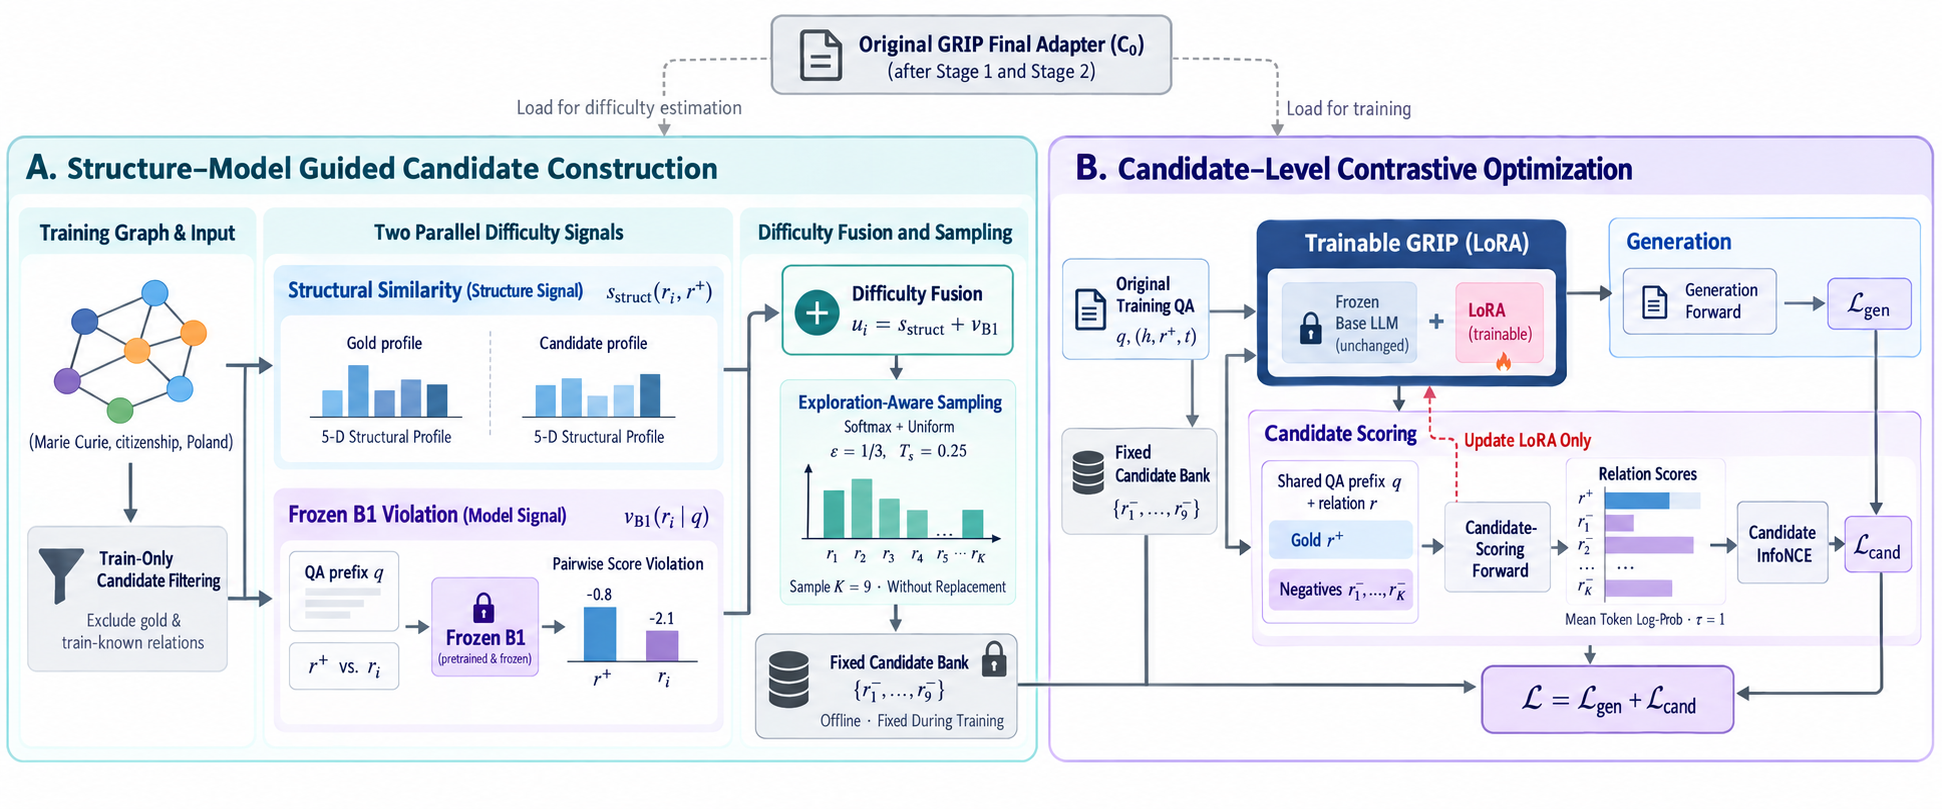
\includegraphics[width=\linewidth]{figures/sccl_structure_guided_svg_content.png}
    \caption{\scc{} 的训练流程。A：训练图关系画像与冻结 \bone{} 分数提供双信号，经过 train-known 过滤与无放回采样，形成每题 $K=9$ 的固定候选库。B：Stage~2 保留原始生成损失，并加入候选级 InfoNCE 共同优化 LoRA。图中损失求和省略了候选权重；严格定义见式~\ref{eq:total}。}
    \label{fig:mechanism}
\end{figure}

图中顶部 $C_0$ 的加载路径为概念性示意：当前实现的 Stage~2 从 Stage~1 adapter 初始化，冻结的 \bone{} 仅用于离线候选评分，不参与训练时的梯度更新。

\subsection{训练图关系画像}

对每一个 $r\in\mathcal{R}_{\mathrm{tr}}$，我们从 $\mathcal{E}_{\mathrm{tr}}$ 计算五维关系画像
\begin{equation}
    \phi(r)=\bigl(\log(1+|E_r|),\log(1+|H_r|),\log(1+|T_r|),
    \overline{d}_{H,r},\overline{d}_{T,r}\bigr),
    \label{eq:profile}
\end{equation}
其中 $|E_r|$ 为关系边数，$|H_r|$ 和 $|T_r|$ 分别为关系覆盖的头实体数与尾实体数，
$\overline{d}_{H,r}$ 是关系边上头实体的平均出度，$\overline{d}_{T,r}$ 是尾实体的平均入度。前两类计数使用 $\log(1+x)$，避免高频关系完全支配距离；度统计保留图的局部连接性。

对目标关系 $r^+$ 和候选 $r$，定义归一化结构相似度
\begin{equation}
    s_{\mathrm{str}}(q,r)=1-\frac{1}{5}\sum_{j=1}^{5}
    \frac{|\phi_j(r^+)-\phi_j(r)|}
    {|\phi_j(r^+)|+|\phi_j(r)|+\epsilon},
    \label{eq:similarity}
\end{equation}
其中 $\epsilon$ 防止两个稀疏特征同时为零。实现将该值裁剪到 $[0,1]$。这个分数只表达“结构画像相近”，不表达两个关系的语义等价性，也不替代对当前实体对的已知关系过滤。

\subsection{冻结 B1 的边界违例度}

\bone{} 是原始 GRIP 的 generation-only 基线。我们在训练问题上离线计算全关系词表的 continuation score。若离线记录已有 pairwise confusion，则直接使用裁剪到 $[0,1]$ 的 confusion；否则对候选和正关系的分数差使用平滑违例度
\begin{equation}
    V_{\bone}(q,r)=\sigma\left(\frac{z_{\bone}(q,r)-z_{\bone}(q,r^+)}{\tau_v}\right).
    \label{eq:violation}
\end{equation}
候选越接近或超过正关系，$V_{\bone}$ 越大。B1 的输出在 bank 构造后冻结，因而 SC-CL 不会把自身训练后的 test 预测反过来用于采样。

\subsection{结构反事实候选分布}

将结构相似度和分数违例度合成为
\begin{equation}
    u(q,r)=\alpha s_{\mathrm{str}}(q,r)+\beta V_{\bone}(q,r),
    \qquad r\in P_q.
    \label{eq:utility}
\end{equation}
候选分布使用均匀下限与 utility softmax 的混合：
\begin{equation}
    p(r\mid q)=\frac{\rho}{|P_q|}+(1-\rho)
    \frac{\exp(u(q,r)/\tau_s)}{\sum_{r'\in P_q}\exp(u(q,r')/\tau_s)}.
    \label{eq:sampling}
\end{equation}
我们从 $p(r\mid q)$ 无放回抽取 $K=9$ 个负关系。默认参数为 $\rho=1/3$、$\alpha=1$、$\beta=1$、$\tau_s=0.25$。如果 $|P_q|<K$，样本进入失败清单而不是静默重复候选；正式实验必须报告该清单及其原因。

这里的“反事实”可写成一个受限操作：在已观测的 $(h,t,r^+)$ 上将标签替换为 $r\in P_q$。$r$ 不是 $T_{\mathrm{tr}}(h,t)$ 中的关系，因此该替换没有复现训练图已知事实；但它仍可能对应真实世界中的未标注事实。这个定义保留了知识图谱的开放世界语义，并让“合法负例”成为数据协议而非未经证实的真值断言。

\subsection{冻结 bank 与候选学习}

SC-CL 的预处理阶段写入每个问题的 question ID、正关系、九个候选、每个候选的结构相似度、违例度、utility、B1 score gap、采样参数、split 和 known-pair 过滤记录。bank manifest 至少满足以下门：

\begin{enumerate}
    \item 所有问题的 \texttt{split} 必须为 \texttt{train}，\texttt{filter\_splits} 只能包含 \texttt{train}；
    \item 每个样本恰有一个正关系和 $K=9$ 个互异候选，候选均属于 $\mathcal{R}_{\mathrm{tr}}$；
    \item 候选与 $T_{\mathrm{tr}}(h,t)$ 不相交，且 question ID 与完整 task JSON 一一对齐；
    \item bank hash、脚本版本、随机种子和结构采样参数被写入 manifest，训练后不得覆盖原文件。
\end{enumerate}

训练时，候选 continuation score 代入式~\ref{eq:infonce}，生成损失仍按原始 GRIP 路径计算。该设计将 SC-CL 的影响集中到“给定候选集合如何区分关系”，而不是同时改变上下文构造或自由解码。

\subsection{复杂度与实现边界}

关系画像只需一次线性扫描训练边，复杂度为 $O(|\mathcal{E}_{\mathrm{tr}}|)$；每个问题的候选 utility 在关系词表上计算，复杂度约为 $O(|\mathcal{R}_{\mathrm{tr}}|)$，采样后 bank 大小为 $O(K|Q_{\mathrm{tr}}|)$。结构画像与采样本身不需要 GPU；冻结 B1 的全关系 continuation scoring 和后续候选训练则需要额外模型计算，实测成本见第 5 节。确定性、过滤和非训练 split 拒绝通过实现测试检查。

\section{实验与结果}

\subsection{设置与评估}

本文评价固定实体对上的十选一关系预测。每题由模型为给定选项生成 continuation score，最高分的关系作为预测；正确率记为官方 Exact Match（EM），同时报告 MRR 和 Hits。数据集、Qwen2.5-7B-Instruct 基座与 GRIP 原论文的设置对应；原论文结果从表 2、表 3 摘录 \citep{feng2025grip}。NELL23K 的 SC-CL 运行使用 seed=2026，完整测试输出包含 4,943 条问题。FB15K237-2 行来自历史 InfoNCE-i0 运行，其候选文件和训练配置与 SC-CL 不同，作为候选对比训练的辅助观察。

\subsection{训练链路与候选库}

NELL23K 候选库由训练问题构造，共 3,253 行，每行九个互异关系，\texttt{rows\_failed=0}。冻结 bank 的 wiring 报告确认训练来源、任务问题对应关系和 manifest 记录。SC-CL Stage~2 完成 10 个 epoch、240 个优化步，并保存 adapter、预测与候选评分。上述记录使候选来源与本次运行可复核。过滤仅排除训练图已知关系；未观测关系的开放世界真值仍需单独审计。

\subsection{主结果}

表~\ref{tab:student-main} 给出两个数据集的官方 EM 与排序指标。NELL23K 上，SC-CL 的官方 EM 为 91.52\%，相对原始 GRIP 论文的 87.74\% 高 3.78 个百分点；MRR 为 95.27\%。FB15K237-2 的历史 InfoNCE-i0 官方 EM 为 91.62\%，相对原始 GRIP 的 88.75\% 高 2.87 个百分点。FB 行不作为 SC-CL 的跨图复现。

\begin{table}[t]
\caption{关系预测结果（百分比；Qwen-7B）。原始 GRIP 数据取自其论文表 2 与表 3。}
\label{tab:student-main}
\centering\scriptsize
\begin{tabular}{llrrrrrr}
\toprule
数据集 & 本地方法 & $n$ & 官方 EM & MRR & H@3 & H@10 & 原始 GRIP EM \\
\midrule
NELL23K & \scc-9 & 4,943 & 91.52 & 95.27 & 99.07 & 100.00 & 87.74 \\
FB15K237-2 & 历史 InfoNCE-i0 & 10,000 & 91.62 & 95.41 & 99.20 & 100.00 & 88.75 \\
\bottomrule
\end{tabular}
\end{table}

同候选的 NELL23K 前 200 条问题另提供本地 \bone{} 配对比较。\scc{} 与 \bone{} 的 EM 分别为 91.00\% 与 88.50\%，MRR 分别为 94.96\% 与 93.36\%。逐题 top-1 变化为九条由错转对、四条由对转错、173 条共同正确和 14 条共同错误。这一前缀子集仅用于分析局部差异，不能替代全量测试。

\subsection{成本与进一步验证}

NELL 运行在训练集上为 644,094 个关系候选生成冻结 B1 分数，用时 19,027 秒，峰值显存为 15.21 GiB。SC-CL Stage~2 处理 12,148,720 个输入 token，用时约 80,870 秒；全测试候选评分用时 3,567 秒。完整的同预算 Random-9 和频率匹配随机对照尚未执行，因此组合采样机制的独立贡献、单位收益成本与多种子稳定性仍需检验。附录~\ref{sec:future-protocol} 说明后续比较协议。

\section{讨论与局限}

\paragraph{候选级学习的解释。}
NELL23K 的官方 EM 为 91.52\%，高于原始 GRIP 论文的 87.74\%。同候选前 200 条问题上，本地 SC-CL 的 MRR 也高于 B1。这些观察与困难候选提供更清晰关系边界的设想相容。不过，前缀子集不能代表完整测试集；结构画像与基线违例度的各自作用还需要单信号消融和匹配训练预算的随机候选对照。

\paragraph{开放世界边界。}
train-known 过滤仅排除训练图中该实体对已有的关系。剩余候选可能在持出 split 或真实世界中成立，因此“结构反事实”是训练标签替换的操作名，不是经过验证的假事实。持出正例重叠与开放世界未判定需要分开统计；CoDEx 的实体替换硬负例也不能为本文的关系替换候选提供真值 \citep{safavi2020codex}。

\paragraph{成本与适用范围。}
冻结 bank 使候选来源可追溯，但需要离线计算 B1 的全关系分数，也不能随训练中的模型更新。现有资源记录只覆盖 NELL23K 的一次运行，尚不能判断收益是否抵消额外成本。方法针对固定实体对上的关系预测；图级组合问答需要重新定义反事实单位和评估目标。跨图适用性仍取决于 FB15K237-2、WN18RR 和 CoDEx-M 上的同契约实验。

\section{结论}

本文提出 SC-CL，在训练关系词表内过滤同一实体对的已知关系，再以结构画像和冻结基线的分数违例度构造九候选库，用于 GRIP Stage~2 的候选级 InfoNCE。固定候选库及其来源记录使训练流程可复核；未观测关系仍保留开放世界中的真值不确定性。

NELL23K 的一次运行在 4,943 条问题上获得官方 EM 91.52\% 和 MRR 95.27\%，超过原始 GRIP 论文报告的 EM 87.74\%。FB15K237-2 的历史候选对比训练实例在 10,000 条问题上获得官方 EM 91.62\%，高于原始 GRIP 的 88.75\%；该实例采用不同训练配置，不构成 SC-CL 的跨图复现。候选来源消融、多种子复现和开放世界冲突审计将进一步检验方法的稳定性与适用范围。


\clearpage
\appendix
\section{补充结果与审计协议}

\subsection{历史 FB 候选评分的来源边界}

\begin{table}[h]
\caption{FB15K237-2 历史十选一评估（百分比，10,000 条测试问题）。InfoNCE-i0 使用历史候选文件和不同训练配置，不是 SC-CL 的跨数据集结果。}
\label{tab:historical-fb}
\centering\scriptsize
\begin{tabular}{lrrrr}
\toprule
方法 & 官方 EM/H@1 & MRR & H@3 & H@10 \\
\midrule
\bone & 79.91 & 88.01 & 95.80 & 100.00 \\
历史 InfoNCE-i0 & 91.62 & 95.41 & 99.20 & 100.00 \\
\bottomrule
\end{tabular}
\end{table}

两组评分均来自相同的本地 processed test，哈希为
\texttt{c77dde51aafc7b1ce3a5011ade914343c2689f8b38b12774ea4840ec1c9068ed}。
历史 i0 使用 \texttt{fb15k237\_i0\_paired\_candidates.json}，LoRA rank 为 24、Stage 2
训练 5 个 epoch、候选损失权重为 0.1；这些条件与本文 SC-CL 的训练契约不一致。

\subsection{后续比较与可证伪规则}
\label{sec:future-protocol}

完整主比较需要相同基座、Stage 1 adapter、任务文件、提示、候选数、候选损失设置和
Stage 2 预算。\bone{} 是原始 generation-only 锚点；Random-9 衡量加入候选损失后的
差异；频率匹配随机检验结构画像是否只是关系频率代理；Profile-only 与 Violation-only
分别检验两个信号，ErrorMemory-9 仅作辅助对照。若 SC-CL 不优于频率匹配随机，组合
采样优势的主张必须撤回；还需单独记录输出格式、未列出的答案与 OOV 情况。

计划在 NELL23K 和 FB15K237-2 上使用训练种子 2026--2030，报告逐种子结果与问题级
配对区间；$K\in\{3,9,15\}$、$\rho\in\{0,1/3,2/3\}$ 和
$\tau_s\in\{0.10,0.25,0.50\}$ 用于敏感性检查。WN18RR 与 CoDEx-M 只有完成任务文本、
adapter、bank 和完整评估的对齐审计后才能进入迁移比较。当前 CoDEx-M 已转换官方正例
split 和固定实体对的关系候选，但 Stage 1/Stage 2 推理及方法训练尚未完成；其通过替换
实体构造的官方硬负例不作为关系候选的真值标签。

每个正式运行需记录 bank 的训练来源、question ID 对齐、每行九个互异候选、train-known
过滤结果、持出正例重叠、数据和 adapter 哈希，以及原始输出与候选评分。
未在训练图出现且未被其他证据确认的候选列为“开放世界未判定”，不计入已证实假阴性。
任何 split 泄漏或任务对齐失败均使该运行退出主比较。

\subsection{默认超参数}

\begin{table}[h]
\caption{SC-CL 的默认设置和正式运行前需要登记的字段。}
\label{tab:hyper}
\centering\small
\begin{tabular}{ll}
\toprule
字段 & 默认值 \\
\midrule
候选数 $K$ & 9 \\
均匀混合系数 $\rho$ & $1/3$ \\
结构权重 $\alpha$ & 1.0 \\
B1 违例权重 $\beta$ & 1.0 \\
采样温度 $\tau_s$ & 0.25 \\
候选损失温度 $\tau_c$ & 运行配置登记 \\
候选损失权重 $\lambda_{\mathrm{cand}}$ & 1.0 \\
bank 随机种子 & 2026 \\
训练种子 & 2026, 2027, 2028, 2029, 2030 \\
过滤来源 & train-only \\
\bottomrule
\end{tabular}
\end{table}

\subsection{候选 bank 的最小 schema}

每一行 bank 至少包含：\texttt{question\_id}、\texttt{split}、\texttt{head}、\texttt{tail}、\texttt{gold\_relation}、
\texttt{negative\_relations}、\texttt{negative\_source}、\texttt{filter\_splits}、\texttt{counterfactual\_operation}、
\texttt{counterfactual\_validation}、\texttt{K}、\texttt{uniform\_mix}、\texttt{structure\_weight}、
\texttt{violation\_weight}、\texttt{temperature}、\texttt{seed} 和 sampler 版本。每个候选记录还应包含
\texttt{structure\_similarity}、\texttt{score\_violation}、\texttt{utility}、\texttt{candidate\_score}、
\texttt{gold\_score}、\texttt{score\_gap} 和 \texttt{counterfactual\_valid}。字段名以项目的实际 JSONL
实现为准，论文只要求这些语义信息可审计。

\subsection{审计伪代码}

\small
\begin{verbatim}
for q in train_questions:
    assert q.split == "train"
    P = train_relations - {q.gold} - known_train_relations(q.head, q.tail)
    for r in P:
        s = profile_similarity(phi[q.gold], phi[r])
        v = b1_score_violation(q, r)
        u[r] = alpha * s + beta * v
    negatives = sample_without_replacement(
        P, mixture_softmax(u, rho, tau), K=9)
    write_frozen_bank(q, negatives, manifest=provenance)
\end{verbatim}

该伪代码强调三个不可省略的顺序：先限定训练 split，再过滤实体对已知关系，最后才计算采样分布。正式 wiring 检查还要确认训练 task 的 question ID、正关系文本和候选关系文本保持一致。

\subsection{失败分类}

\begin{table}[h]
\caption{建议的失败分析标签。}
\label{tab:failure}
\centering\scriptsize
\begin{tabular}{p{0.23\linewidth}p{0.65\linewidth}}
\toprule
标签 & 判定规则 \\
\midrule
结构稀疏 & 目标关系或候选关系的画像特征大部分为零，profile 相似度不稳定。 \\
已知关系冲突 & 候选属于当前实体对 train-known 关系，说明过滤或 bank 版本错误。 \\
开放世界不确定 & 候选未在训练图出现，但在外部/测试事实中可能成立，不能当作确定假阴性。 \\
B1 高置信混淆 & 候选 score 高于 gold，且模型对该关系赋予较高置信度。 \\
候选不足 & 过滤后 $|P_q|<9$，必须进入失败清单，不能重复填充。 \\
输出格式异常 & 模型输出不属于题目给出的关系选项。 \\
\bottomrule
\end{tabular}
\end{table}

\subsection{伦理与数据说明}

本文使用本地知识图谱基准和公开模型技术报告作为背景，不新增个人敏感数据。当前正文
只把带有原始预测、配置、manifest 和 hash 的 NELL 单种子结果作为实测；历史 FB
InfoNCE-i0 另行标注，未完成协议不用于性能承诺。正式提交前应补充数据许可、模型许可
证、代码版本和可公开的 bank/预测文件说明。



\bibliographystyle{iclr2026_conference}
\bibliography{references}

\end{document}
